% !TeX root = ../relazione.tex

\chapter{Implementazione}


\section{Data tier}
Questo modulo comprende il database, per il quale è stato scelto \textbf{MariaDB},
una soluzione open source sviluppata dagli autori di MySQL, e lo sviluppo delle
API per poter stabilire facilmente una connessione con esso ed effettuare
modifiche e interrogazioni, mappando quelle che si definiscono operazioni
\textbf{CRUD} (Create, Retrieve, Update e Delete).

\paragraph{Pattern DAO}
Per l'implementazione si è utilizzato \textbf{Java} come linguaggio di programmazione
e il \textbf{Design Pattern DAO} (Data Access Object) \cite{J2EE-design-patterns}.
Per ogni entità del database sono state quindi definite:
\begin{itemize}
	\item Una classe \textbf{DTO} (Data Transfer Object), che rappresenta la
	relativa entità e le cui istanze vengono utilizzate per lo scambio dei dati
	con il database
	\item Un'interfaccia \textbf{DAO} che definisce i metodi che si possono
	utilizzare per interagire con la relativa entità del database, tra cui le
	operazioni CRUD necessarie
	\item Almeno una classe che implementi il DAO, responsabile dell'effettiva
	connessione con il database e della logica con cui i metodi accedono ai dati
\end{itemize}

\lstinputlisting[language=Java, caption=Interfaccia DAO relativa all'entità \textit{user}]{assets/code/UserDAO.java}

Questa struttura migliora ulteriormente la modularità e la flessibilità del
progetto (v. \autoref{sec:architettura}), in quanto l'Application tier può
fare affidamento solamente sui metodi esposti dall'interfaccia DAO, ignorando quale
sia la specifica implementazione.
In questo modo se ad esempio fosse necessario utilizzare una diversa tecnologia
per il database sarebbe sufficiente una nuova implementazione del DAO, che
manterrebbe gli stessi metodi e non necessiterebbe quindi di effettuare ulteriori
modifiche di adattamento.

\paragraph{Project Lombok}
Una libreria open source che è stata molto utilizzata per ridurre i tempi di
scrittura e migliorare la leggibilità del codice è \textbf{Project Lombok};
un \textit{Annotation processor} che, tramite delle annotazioni nel codice,
sostituisce la scrittura di metodi molto comuni e simili tra loro (come
\textit{setter} o \textit{getter}).
Nelle classi che rappresentano dei dati, come le classi DTO, questo è stato
essenziale per poter scrivere in poche righe un codice chiaro e funzionale;
ad esempio, la classe \texttt{User} (v. \ref{code:user-dto}), grazie alle annotazioni
\texttt{@Getter}, \texttt{@Builder} e \texttt{@Setter}, dispone di metodi get
per ogni campo, di un'implementazione del pattern Builder e di un metodo set per
il campo \texttt{id}.

\lstinputlisting[language=Java, label={code:user-dto}, caption=Classe DTO relativa all'entità \textit{user}]{assets/code/UserDTO.java}



\section{Application tier}
In questo modulo viene gestita la parte logica ed applicativa della piattaforma,
tra cui il controllo della sessione utente e i vincoli derivanti dai requisiti;
come ad esempio la possibilità di accedere ad alcune funzionalità solo per certe
tipologie di utenti o il controllo per cui i link di download siano validi solo
per le richieste approvate e solo per l'utente che ha effettuato la richiesta. 


\subsection{Il framework Spring}
Il linguaggio utilizzato è \textbf{Java} accoppiato a \textbf{Spring},
un framework per lo sviluppo di applicazioni web, nello specifico nella versione
\textbf{Boot} \cite{spring:boot}, che ne semplifica la configurazione e garantisce
la possibilità di avere un web server \textit{stand-alone} direttamente eseguendo
la classe principale del progetto o effettuandone la build, che produrrà un file
JAR eseguibile con la stessa funzionalità.

\paragraph{Services} \label{par:spring-services}
Per la gestione dell'invio delle email, della generazione del modulo pdf e
dell'interazione con il file system per salvatare i moduli inviati e permettere
il download delle risorse, sono state definite delle classi annotate come
\texttt{@Service}, ovvero relative solo a parte della \textit{business logic}
dell'applicazione. I Service vengono poi utilizzati nel resto del progetto
tramite la \textbf{Dependency Injection} di Spring, che si occupa di fornire la
stessa istanza a tutti i componenti che ne richiedono l'utilizzo. La forma di
injection applicata è quella tramite il costruttore della classe 
(v. \ref{code:constr-inj}) che viene parametrizzato automaticamente dal framework
all'avvio dell'applicazione.

\lstinputlisting[language=Java, label={code:constr-inj}, caption=Esempio di Constructor Injection per \texttt{EmailService}]{assets/code/AuthenticationController.constructor.java}

\paragraph{Controllers}
Tra i componenti principali del framework troviamo le classi Controller, definite
tramite l'annotazione \texttt{@RestController} e adibite ad eseguire le funzionalità
nel rispetto dei vincoli dell'applicazione. I metodi di queste classi vengono
mappati a degli endpoint del web server che permettono la loro invocazione tramite
richieste HTTP, creando così delle API accessibili tramite l'interfaccia utente.

Ad esempio nella classe \texttt{AuthenticationController} è stato implementato un
metodo \texttt{signUp} (v. \ref{code:auth-controller-signup}) che permette di
effettuare la registrazione di un nuovo utente. Questo metodo, tramite
l'annotazione \texttt{@PostMapping}, è accessibile effettuando una richiesta POST
all'endpoint \textit{/signup}.

Nel dettaglio, effettua dei controlli sulla validità dei parametri e sull'unicità
di username e indirizzo email, per poi istanziare un nuovo oggetto \texttt{User},
inviare un'email di conferma tramite il Service (v. \autoref{par:spring-services})
che gestisce le email, inserire l'utente nel database tramite un oggetto DAO e
infine associare un nuovo \texttt{AccessToken} all'utente per garantirgli la sessione.

\lstinputlisting[language=Java, label={code:auth-controller-signup}, caption=Metodo \texttt{signUp} della classe \texttt{AuthenticationController}]{assets/code/AuthenticationController.signup.java}

\paragraph{Filters}
La validità delle sessioni utente e l'accesso alle funzionalità riservate per
utenti amministratori o gestori, sono state gestite tramite dei pattern negli
endpoint; utilizzando ad esempio \textit{/api/admin} come prefisso per tutti
quelli su cui era necessario verificare che l'utente fosse un amministratore
(v. \ref{code:admin-filter}).

Definendo delle classi che estendono \texttt{OncePerRequestFilter} è stato
possibile implementare dei controlli eseguiti prima di ogni richiesta che rispetti
il pattern specificato, ritornando un codice di errore nel caso le condizioni
non vengano soddisfatte o permettendo l'esecuzione della richiesta altrimenti.

\lstinputlisting[language=Java, label={code:admin-filter}, caption=Filtro per verificare che l'utente possa accedere ad un endpoint riservato]{assets/code/AdminFilter.java}



\section{Presentation tier}

In questo modulo è stata implementata la \textbf{UI} (User Interface), ovvero il
mezzo di comunicazione tra l'utente finale e i moduli precedenti. In questo caso
si tratta di pagine web che presentano le informazioni e guidano l'utente nell'utilizzo
delle funzionalità della piattaforma; che equivalgono a delle richieste HTTP
inviate all'Application tier e a delle conseguenti risposte di conferma o di errore.


\subsection{Approccio component based}
Per lo sviluppo si è scelta una logica basata su componenti applicata al
paradigma object-oriented, implementata utilizzando \textbf{TypeScript}.
L'approccio utilizzato è quindi quello di sviluppare delle classi che rappresentino
un elemento dinamico dell'interfaccia, a cui è delegata la generazione della propria
struttura HTML, la definizione dello stile grafico CSS e della logica che permette
di svolgere una specifica funzionalità.

È stata quindi definita una classe astratta \texttt{AbstractWidget} per rappresentare
i comportamenti comuni di ogni componente della UI, come ad esempio il modo in cui
vengono mostrati eventuali messaggi di errore o in cui viene gestito lo stato di
attesa di dati da parte del server.

\paragraph{TypeScript}
La scelta di TypeScript \cite{typescriptlang} è ormai quasi uno standard nell'ambito dello sviluppo web.
Si tratta di un linguaggio di programmazione open-source che estende la sintassi
di JavaScript, rendendo compatibile il codice scritto con quest'ultimo per il
compilatore TypeScript. La compilazione in questo caso (detta anche
"transpilazione") produce infatti codice JavaScript.
Il motivo per cui viene utilizzata questo linguaggio è dovuto alla caratteristica
di JavaScript per cui non vengono effettuati controlli statici sui tipi di dato,
che vengono convertiti implicitamente. Anche se questa caratteristica è stata uno
dei motivi del suo successo, la mancanza di controlli all'atto della compilazione
rende più difficile trovare degli errori, sopratutto quando si sviluppano
applicazioni di grandi dimensioni o complessità.
Tra i motivi principali per utilizzare TypeScript troviamo quindi:
\begin{itemize}
	\item Possibilità di annotare i tipi di dato con controllo in fase di compilazione
	\item Inferenza di tipo (type-inference)
	\item Aggiunta delle interfacce
	\item Aggiunta degli enum
	\item Aggiunta dei tipi generici
\end{itemize}


\subsection{Richieste AJAX}
Per effettuare lo scambio di dati con l'Application tier, e quindi le richieste
alle API HTTP, è stato adottato un approccio asincrono tramite richieste
\textbf{AJAX} (Asynchronous JavaScript and XML). Questo significa che la richiesta
non sarà bloccante per l'interfaccia e che i dati saranno aggiornati nel momento
in cui arriverà la risposta dal server, senza esplicito ricaricamento della pagina
web. Nello specifico ogni componente gestisce e mostra un proprio stato di attesa,
così che al completamento delle richieste effettuate si aggiorni dinamicamente in
base al responso del server.

Oltre che per semplificare la creazione e la manipolazione degli elementi HTML
all'interno dei componenti, è stata utilizzata la libreria jQuery \cite{jquery}
anche per effettuare le richieste AJAX, garantendo la compatibilità cross-browser.

\paragraph{Le Promise in JavaScript}
Per gestire le molteplici richieste da dover effettuare, è stata definita una
funzione generica \texttt{apiRequest}, che prende come parametri l'url dell'endpoint
a cui effettuare la richiesta e un oggetto facoltativo per specificare eventuali
parametri richiesti dalle API. Ad ogni richiesta viene aggiunto il token relativo
alla sessione come header di autorizzazione e aggiornato con quello che si riceve
nella risposta del server.
Questa funzione ritorna una \textbf{Promise} \cite{mdn:promise}, ovvero un oggetto
che rappresenta un'operazione che non è stata ancora completata, utile per gestire
computazioni asincrone. La richiesta AJAX all'interno del costruttore viene eseguita
contemporaneamente alla creazione della Promise, associando il valore ritornato
dal server in caso di successo alla funzione \texttt{resolve} o l'eventuale
errore alla funzione \texttt{reject}.
In questo modo i widget che necessitano di effettuare delle richieste API,
possono utilizzare una funzione specifica che si occupa di effettuare la richiesta
AJAX, mentre per gestirne il risultato sarà sufficiente utilizzare i metodi
\texttt{.then()} e \texttt{.catch()} della Promise ritornata, rispettivamente per
il caso di successo e il caso di errore. Entrambi i metodi
prendono come parametro una funzione che verrà eseguita nel momento in cui
l'operazione sarà completata, in questo caso a seguito della risposta del server.

\lstinputlisting[language=Java, caption=Funzione \texttt{apiRequest} per effettuare le richieste AJAX]{assets/code/requests.apirequest.ts}


\subsection{Le pagine realizzate}
Per quanto riguarda lo stile delle pagine e dei widget è stato utilizzato Bootstrap
principalmente per garantire un design responsive tramite il grid-system \cite{bootstrap:grid}
e per alcune classi CSS relative agli elementi più semplici dell'interfaccia.
Inoltre, ad ogni widget è stato associato un file SASS, ovvero un'estensione del
classico CSS, per definire gli stili più specifici.

\subsubsection{Autenticazione e registrazione}
Le schermate e i widget per l'autenticazione e la registrazione implementano un
form e la relativa richiesta AJAX. La struttura dei due widget è condivisa, di
modo che il bottone per passare da una vista all'altra sia sempre la label sulla
sinistra, mentre sulla destra ci sia sempre quello per effettuare l'azione.

Una volta autenticati, si viene reindirizzati alla successiva schermata in base
alla tipologia di utente, così che un utente web possa direttamente selezionare
le risorse per cui richiedere accesso (v. \autoref{subsec:resources-selection}),
mentre un utente gestore o amministratore possa avere da subito una panoramica
sulle richieste (v. \autoref{subsec:submissions-list}).

\begin{figure}[H]
	\centering
	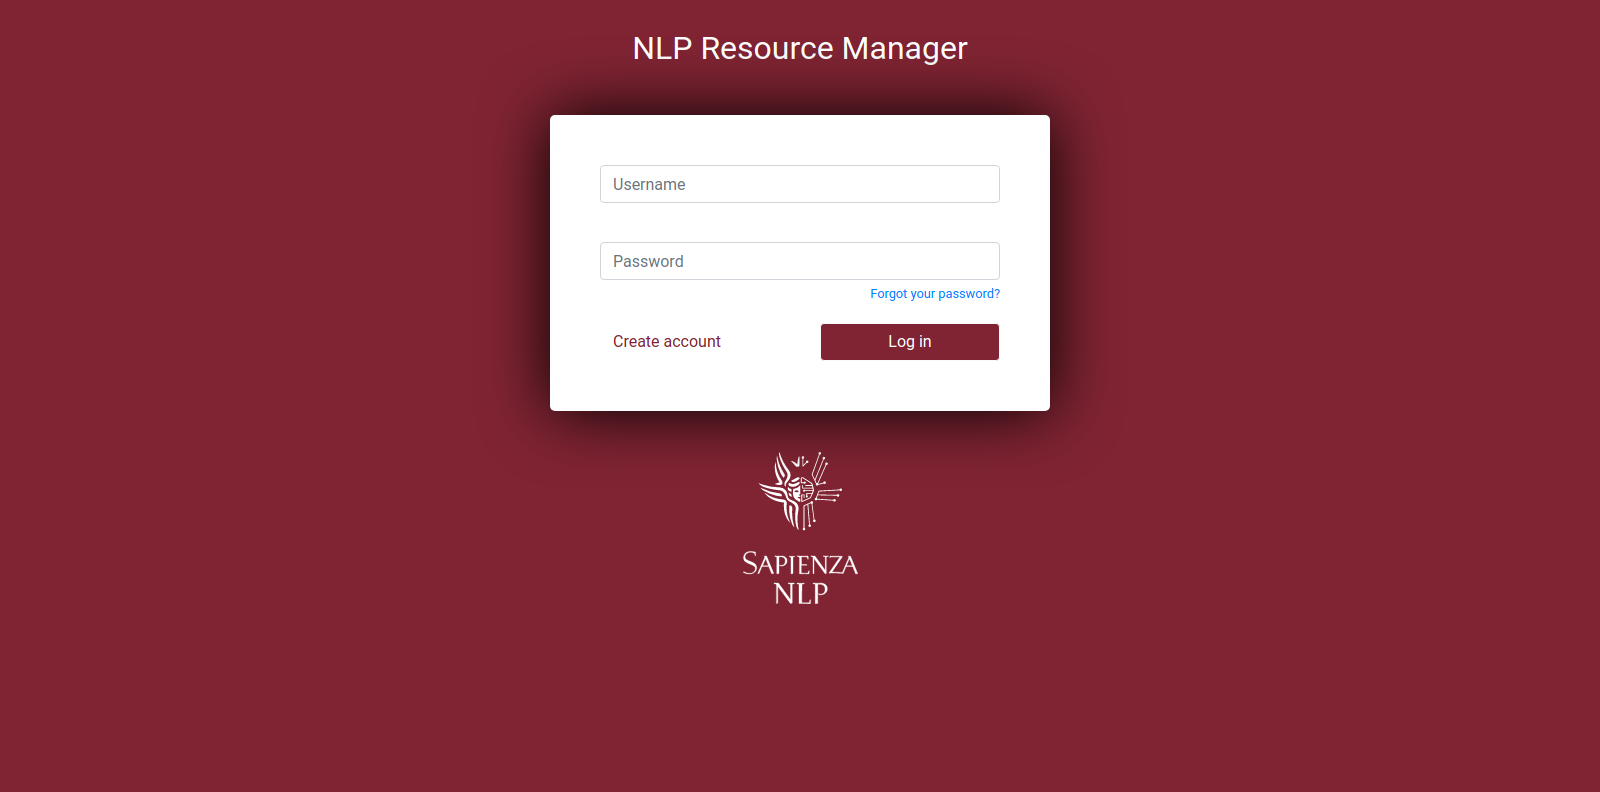
\includegraphics[width=\textwidth]{assets/ui/login.png}
	\caption{Autenticazione}
	\label{fig:login}
\end{figure}

\begin{figure}[H]
	\centering
	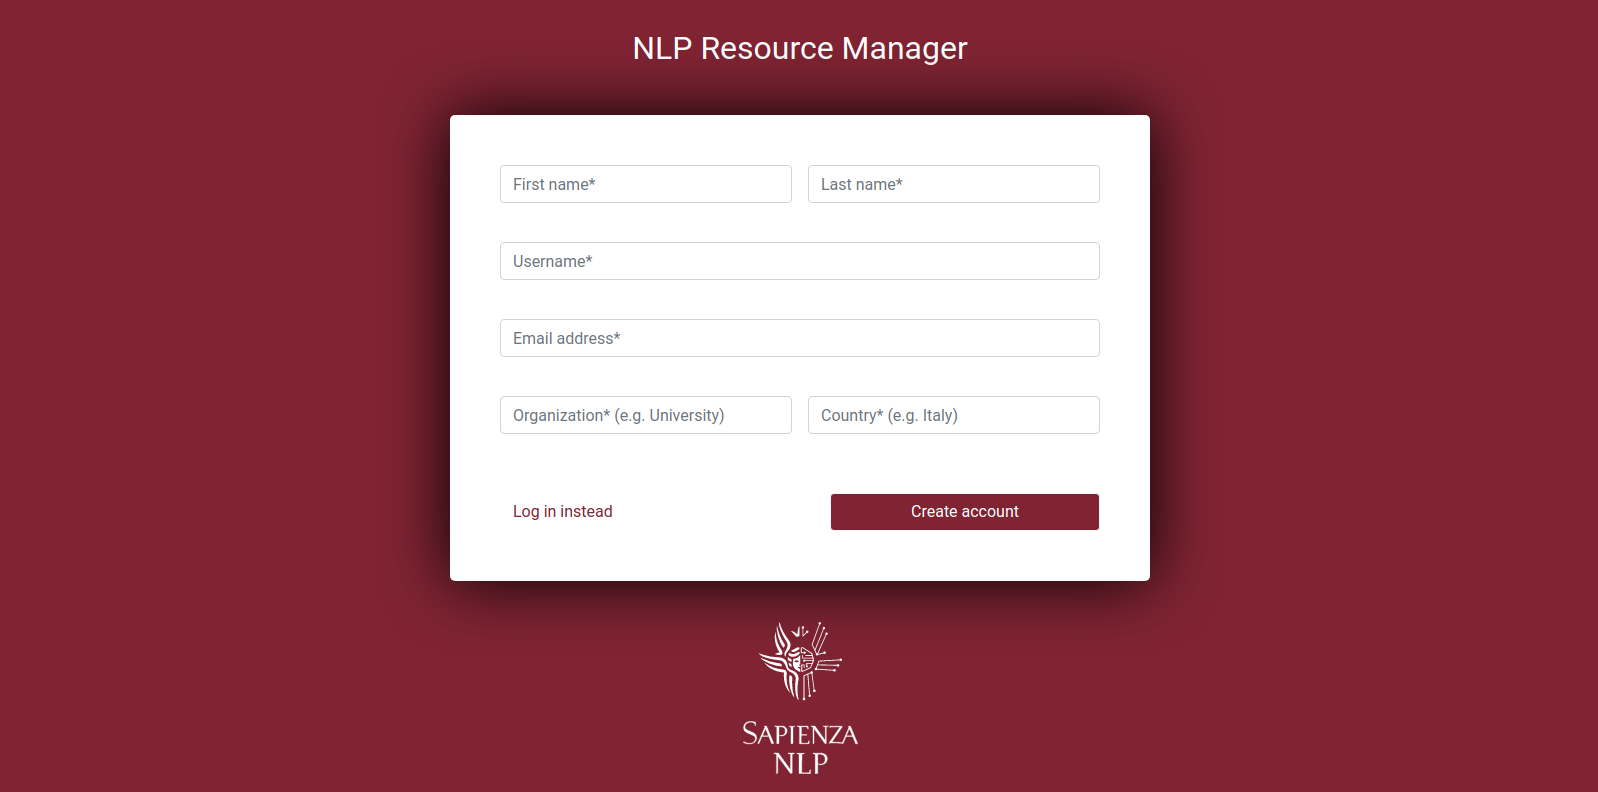
\includegraphics[width=\textwidth]{assets/ui/signup.png}
	\caption{Registrazione}
	\label{fig:signup}
\end{figure}

\subsubsection{Selezione delle risorse} \label{subsec:resources-selection}
Come in tutte le altre schermate della home, l'interfaccia è divisa in due parti,
con sulla sinistra una sidebar placeholder con i riferimenti Sapienza e sulla
destra il widget principale. In questa schermata il widget si occupa di richiedere
e mostrare la lista di tutte le risorse disponibili, oltre che di gestirne la
selezione multipla e il filtro per parola chiave tramite la barra di ricerca.
L'inserimento della descrizione relativa all'utilizzo previsto è gestito dallo
stesso, con una transizione delle informazioni mostrate e dei bottoni disponibili.

Una volta confermata l'operazione, viene effetuata una richiesta che, in caso di
conferma, ritorna il modulo pdf da dover firmare, scaricato automaticamente dal
client. L'upload del pdf firmato sarà poi possibile dalla schermata successiva
(v. \autoref{subsec:pdf-upload}), accessibile dal menù di navigazione in alto.

\begin{figure}[H]
	\centering
	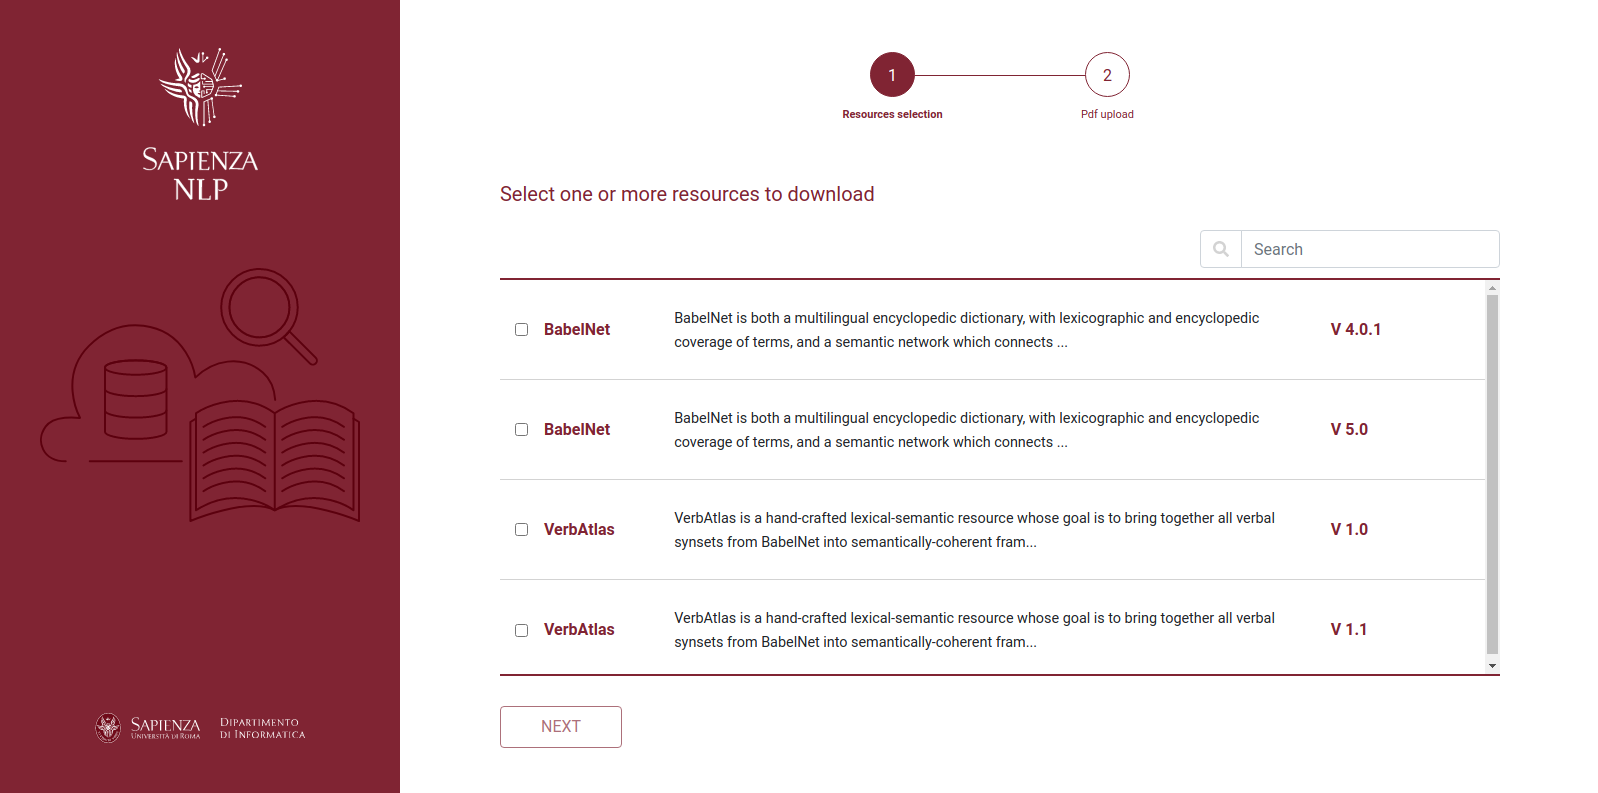
\includegraphics[width=\textwidth]{assets/ui/resources-selection.png}
	\caption{Selezione delle risorse}
	\label{fig:resources-selection}
\end{figure}

\begin{figure}[H]
	\centering
	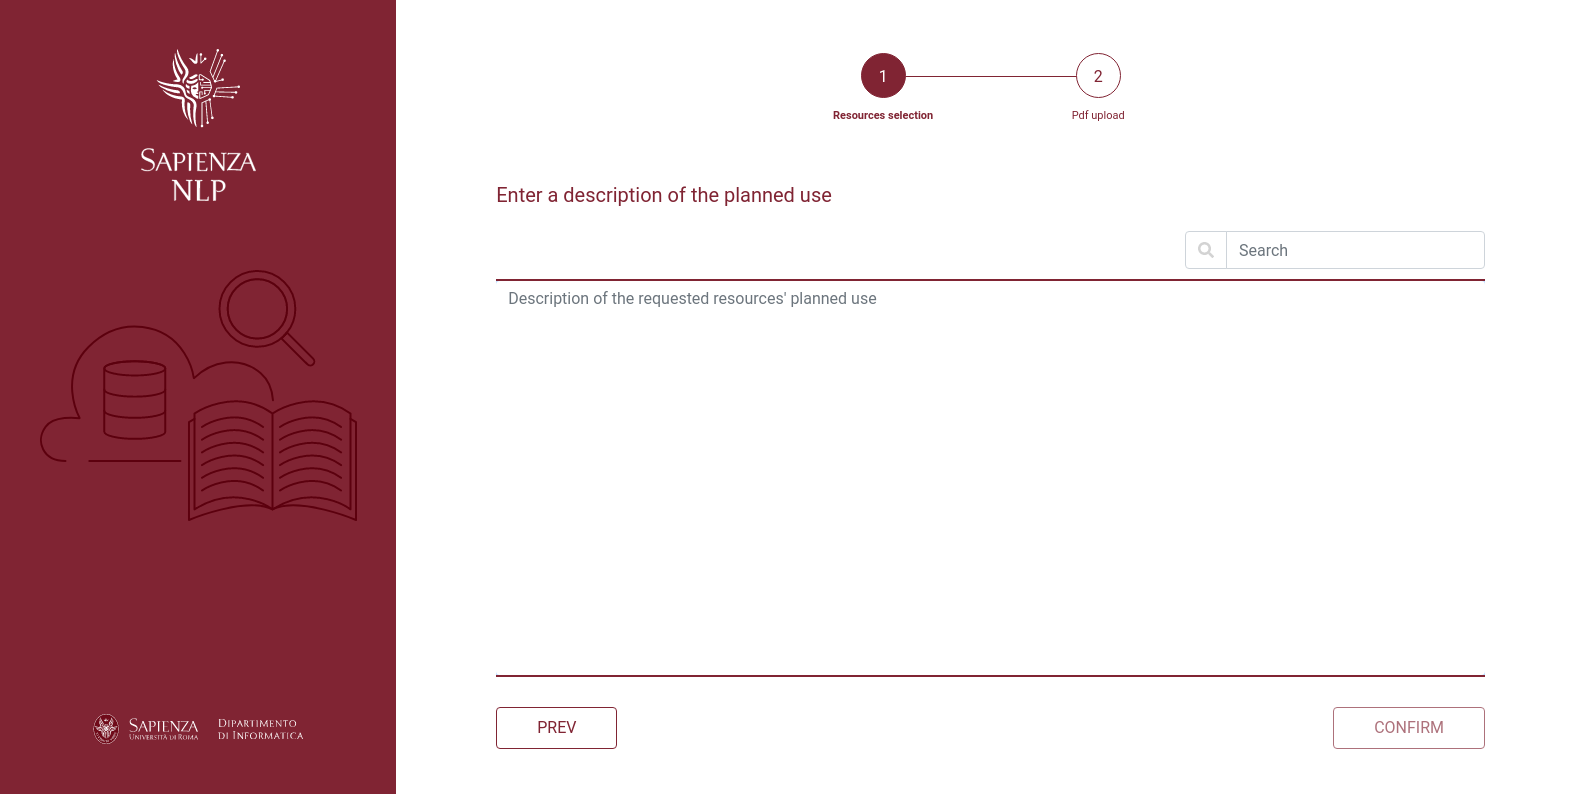
\includegraphics[width=\textwidth]{assets/ui/request-description.png}
	\caption{Inserimento descrizione dell'utilizzo}
	\label{fig:request-description}
\end{figure}

\subsubsection{Upload del modulo pdf firmato} \label{subsec:pdf-upload}
L'ultimo passo per richiedere l'accesso alle risorse è quello di effettuare
l'upload del modulo pdf firmato. Questa operazione è stata implementata con un
widget per gestire anche il drag and drop e i controlli sulla tipologia e sulla
dimensione del file. Una volta effettuato il \textit{submit}, il server si occupa
in ogni caso di controllare che il file sia in un formato valido e che contenga
dei metadati di validazione e, in caso di successo, il client mostra una
schermata di conferma (v. \autoref{fig:request-success}).

\begin{figure}[H]
	\centering
	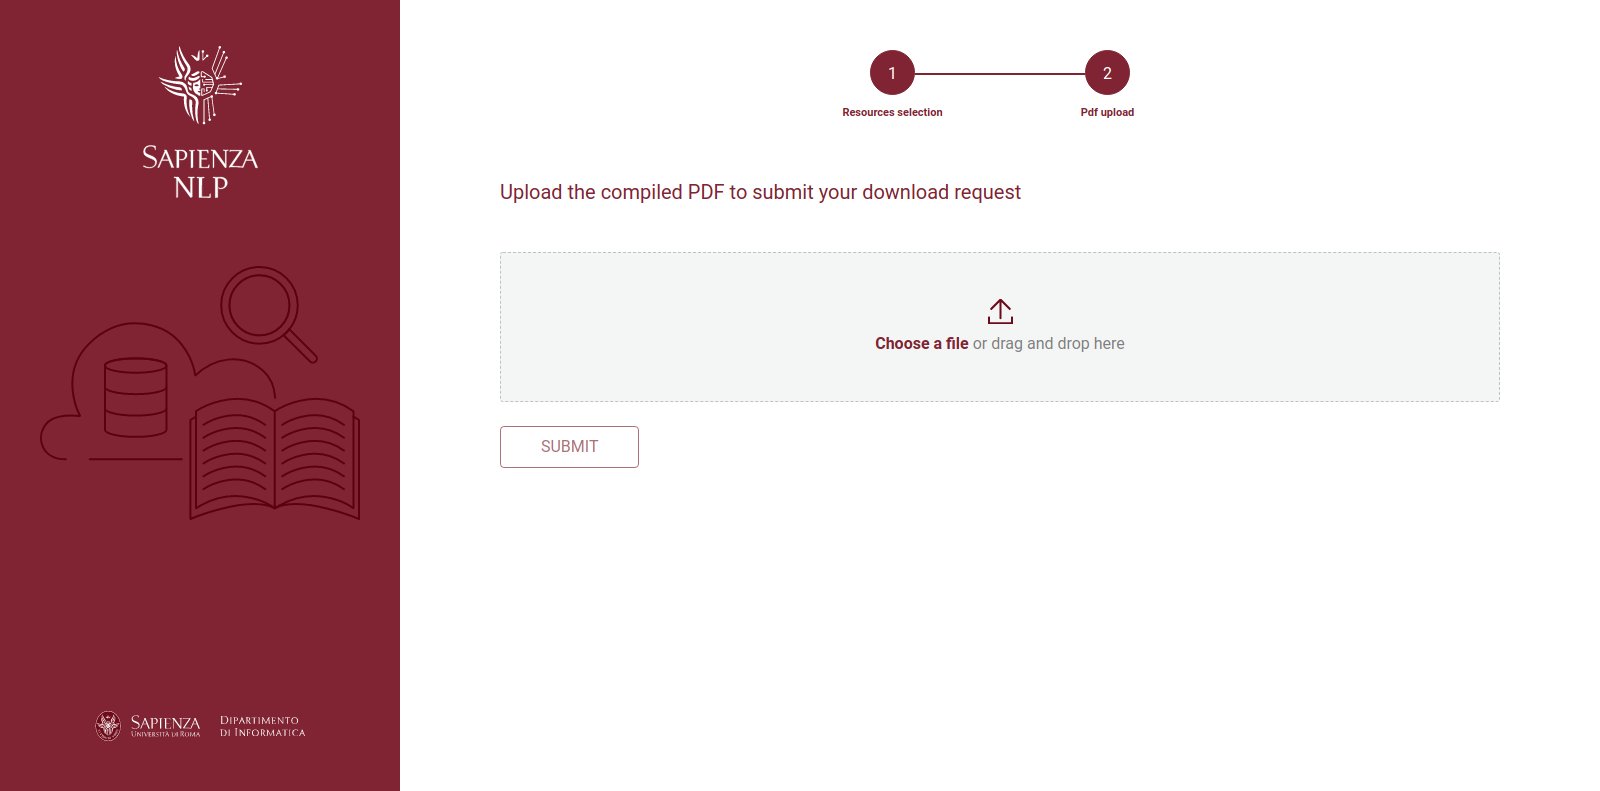
\includegraphics[width=\textwidth]{assets/ui/pdf-upload.png}
	\caption{Upload modulo pdf firmato}
	\label{fig:pdf-upload}
\end{figure}

\begin{figure}[H]
	\centering
	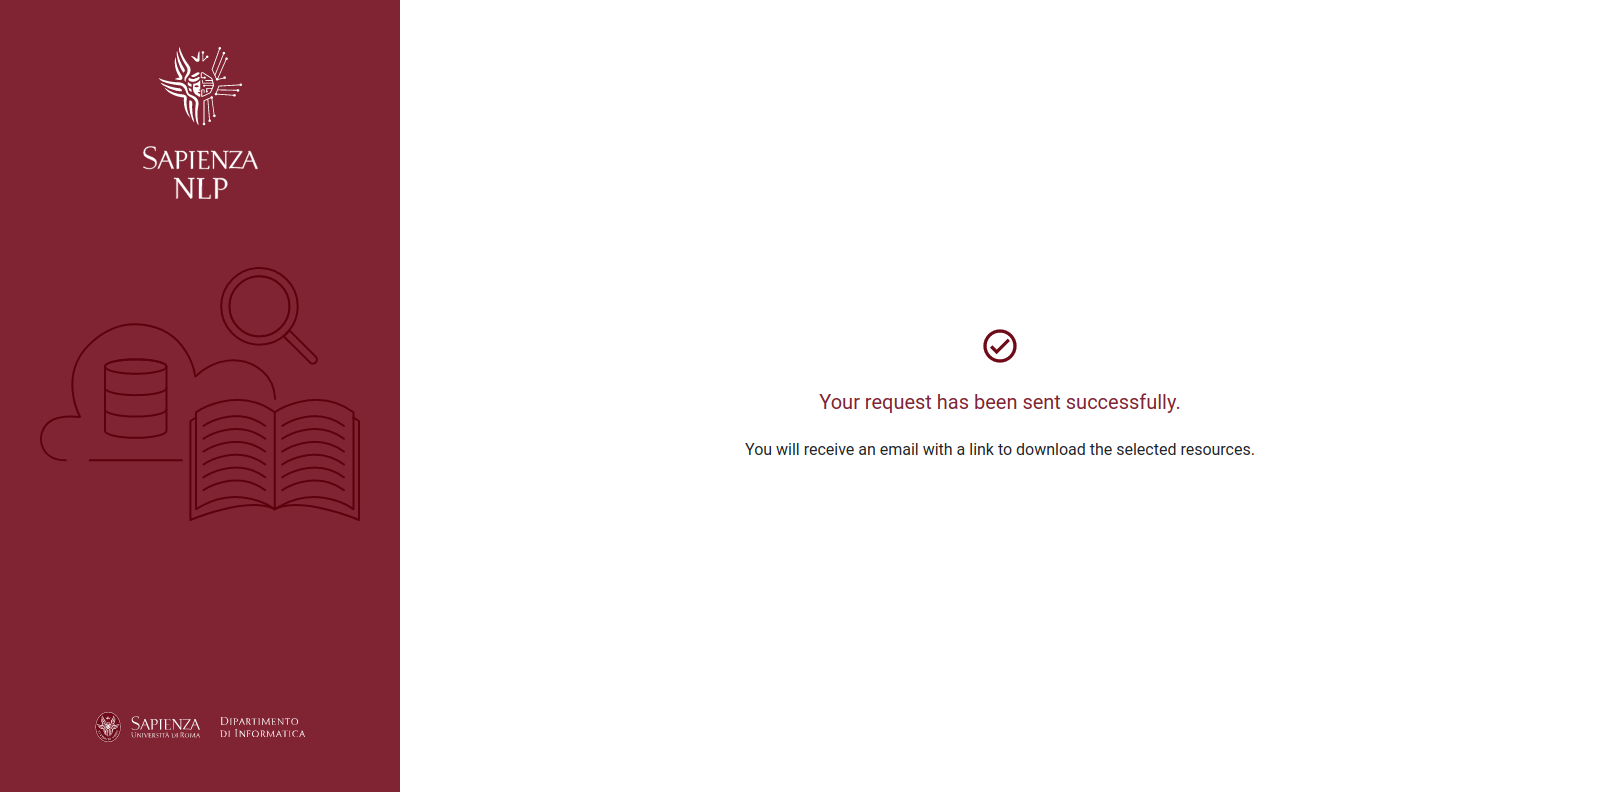
\includegraphics[width=\textwidth]{assets/ui/request-success.png}
	\caption{Conferma completamento richiesta}
	\label{fig:request-success}
\end{figure}

\subsubsection{Gestione delle richieste effettuate} \label{subsec:submissions-list}
Nelle schermate di amministrazione l'interfaccia perde la sidebar presente nella
home in favore di una barra di navigazione che permette di accedere alle varie
sezioni del pannello. L'accesso è limitato a soli utenti autorizzati e in caso
il server notifichi una violazione si viene reindirizzati alla schermata di
autenticazione. In questo caso sono presenti più widget, ognuno assolve una
diversa funzionalità, per cui è possibile:
\begin{itemize}
	\item Visualizzare tutte le richieste effettuate, con la data di sottomissione
	lo stato attuale e un bottone per aprirne il dettaglio (v. \autoref{fig:submissions-list})
	\item Visualizzare i dettagli della richiesta, con la possibilità di
	modificarne lo stato e di visualizzare il modulo pdf caricato dall'utente (v. \autoref{fig:submission-details})
	\item Visualizzare lo storico dei cambiamenti di stato, con il relativo utente
	che ha effettuato l'operazione (v. \autoref{fig:submission-details})
	\item Visualizzare la lista delle risorse associate alla richiesta, con la
	possibilità di selezionare per quali generare i link di download (v. \autoref{fig:submission-details})
\end{itemize}

\begin{figure}[H]
	\centering
	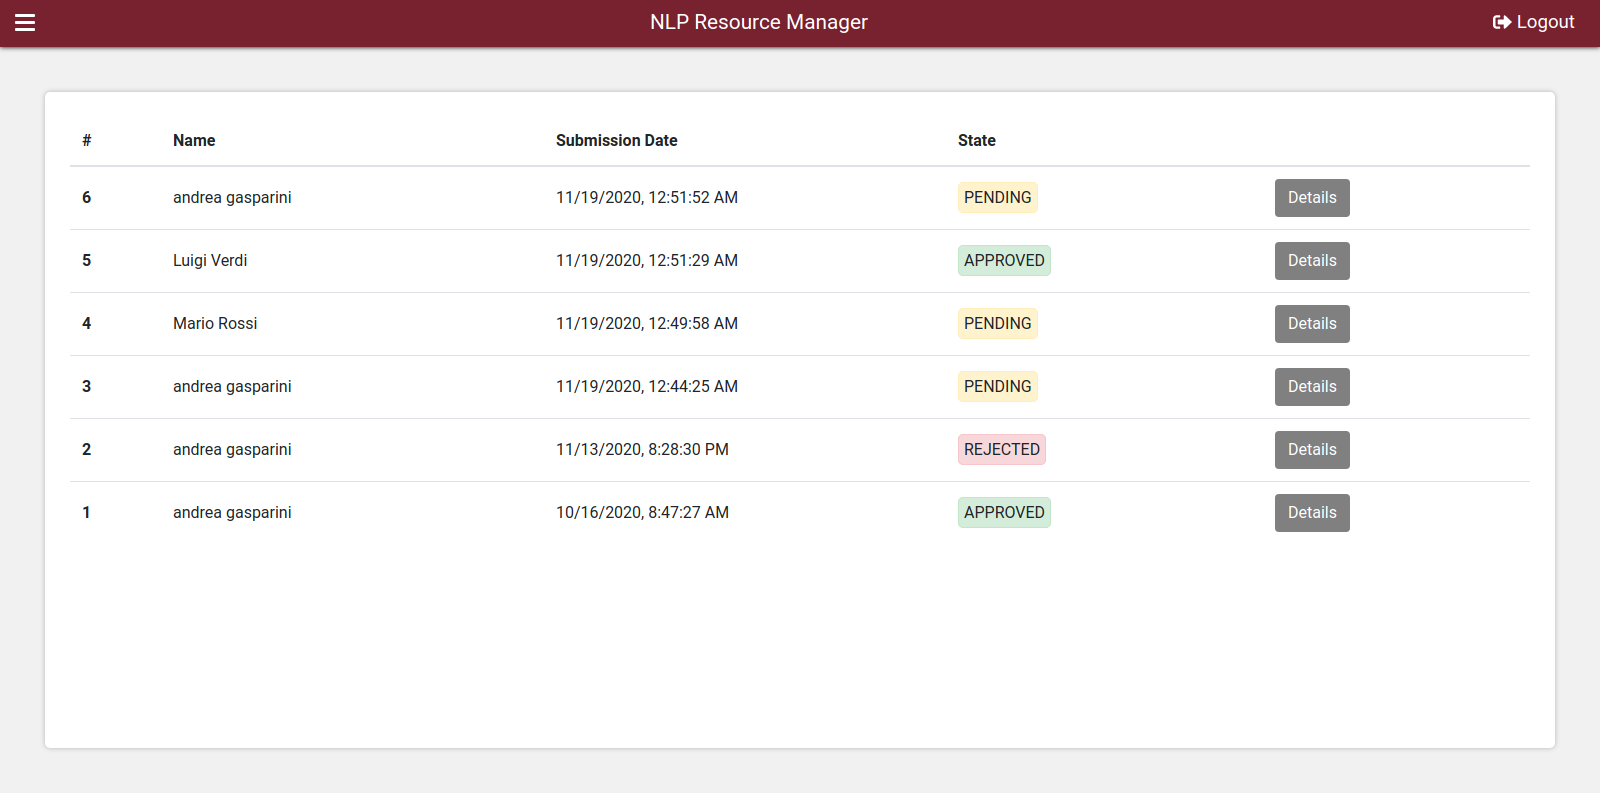
\includegraphics[width=\textwidth]{assets/ui/submissions-list.png}
	\caption{Resoconto di tutte le richieste effettuate}
	\label{fig:submissions-list}
\end{figure}

\begin{figure}[H]
	\centering
	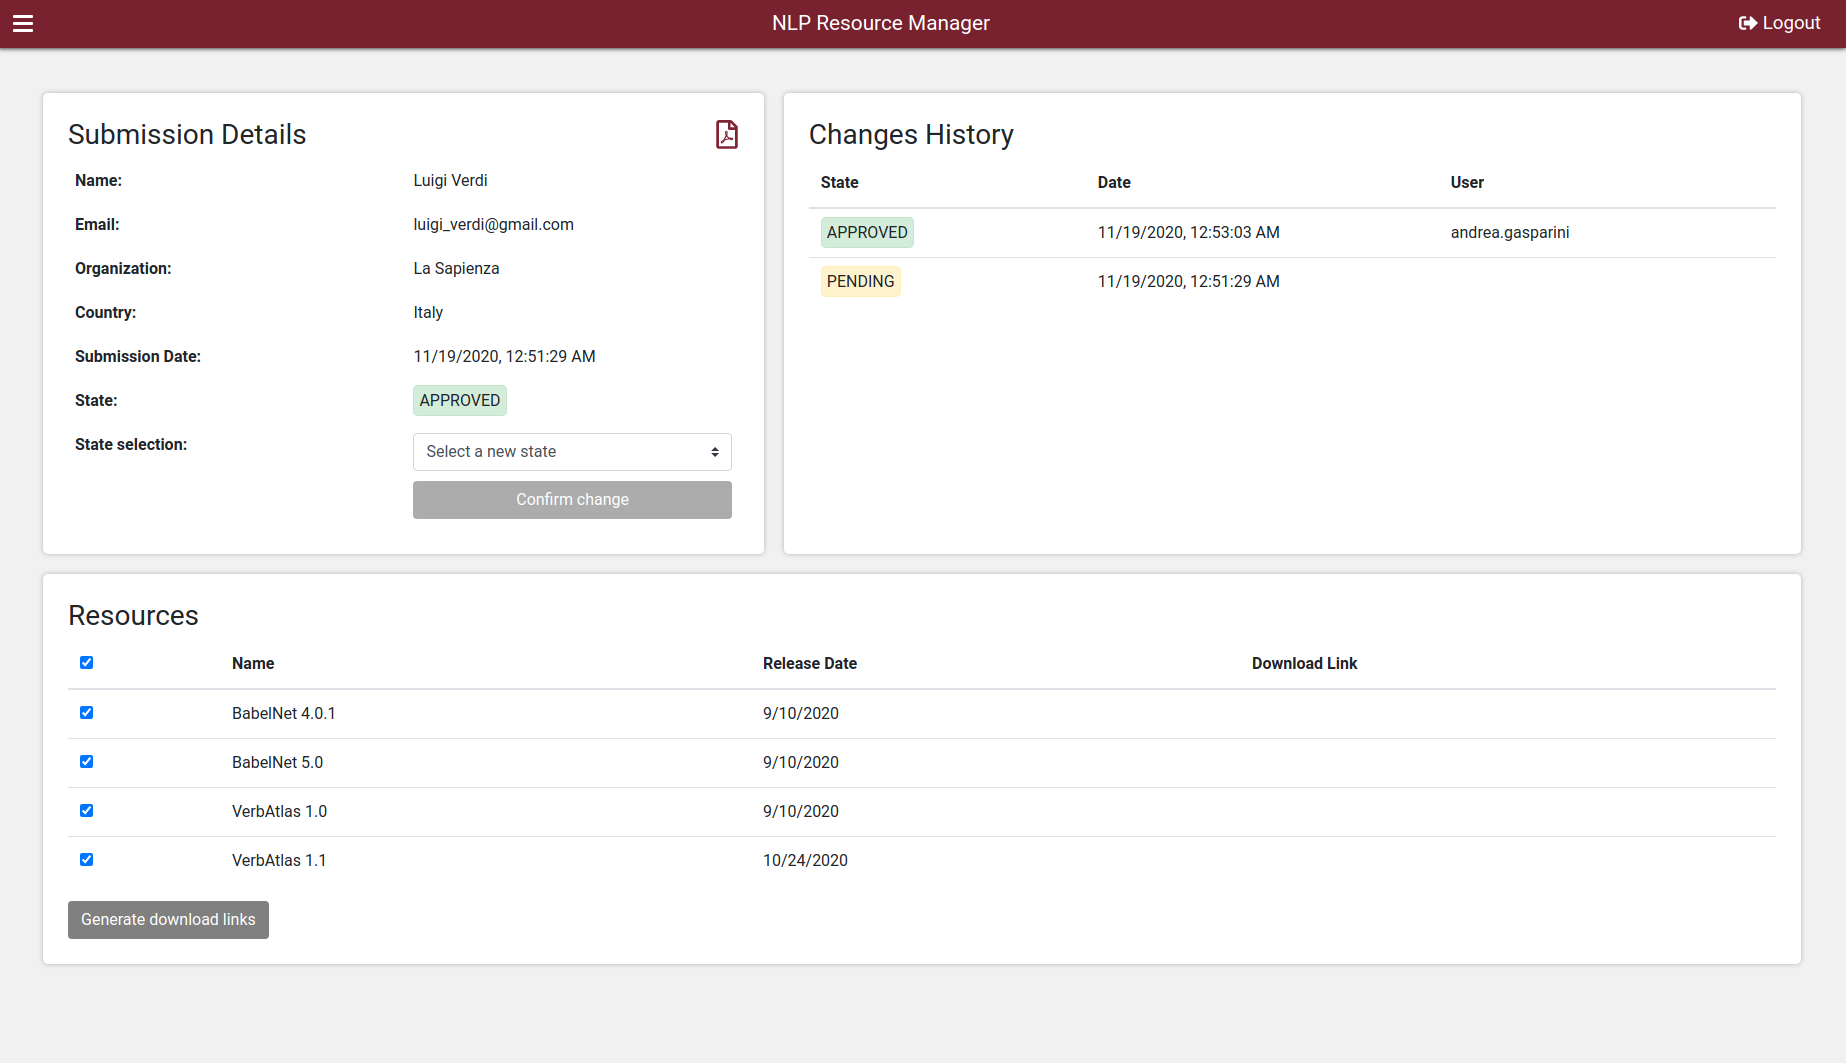
\includegraphics[width=\textwidth]{assets/ui/submission-details.png}
	\caption{Dettaglio di una richiesta effettuata}
	\label{fig:submission-details}
\end{figure}

\subsubsection{Gestione degli utenti}
In queste schermate di amministrazione è possibile visualizzare un resoconto di
tutti gli utenti registrati e di aprirne un dettaglio, in cui è possibile modificarne
i dati e visualizare la cronologia delle azioni effettuate (richieste sottomesse
o cambi di stato in base alla tipologia di utente). Per il widget relativo alla
cronologia è stato riutilizzato quello già presente nel dettaglio delle richieste
grazie all'approccio modulare basato su componenti che favorisce il riuso del codice.
Allo stesso modo, per creare un nuovo utente viene utilizzando lo stesso widget
che in \autoref{fig:user-details} permette la modifica dei dati di uno già esistente.

\begin{figure}[H]
	\centering
	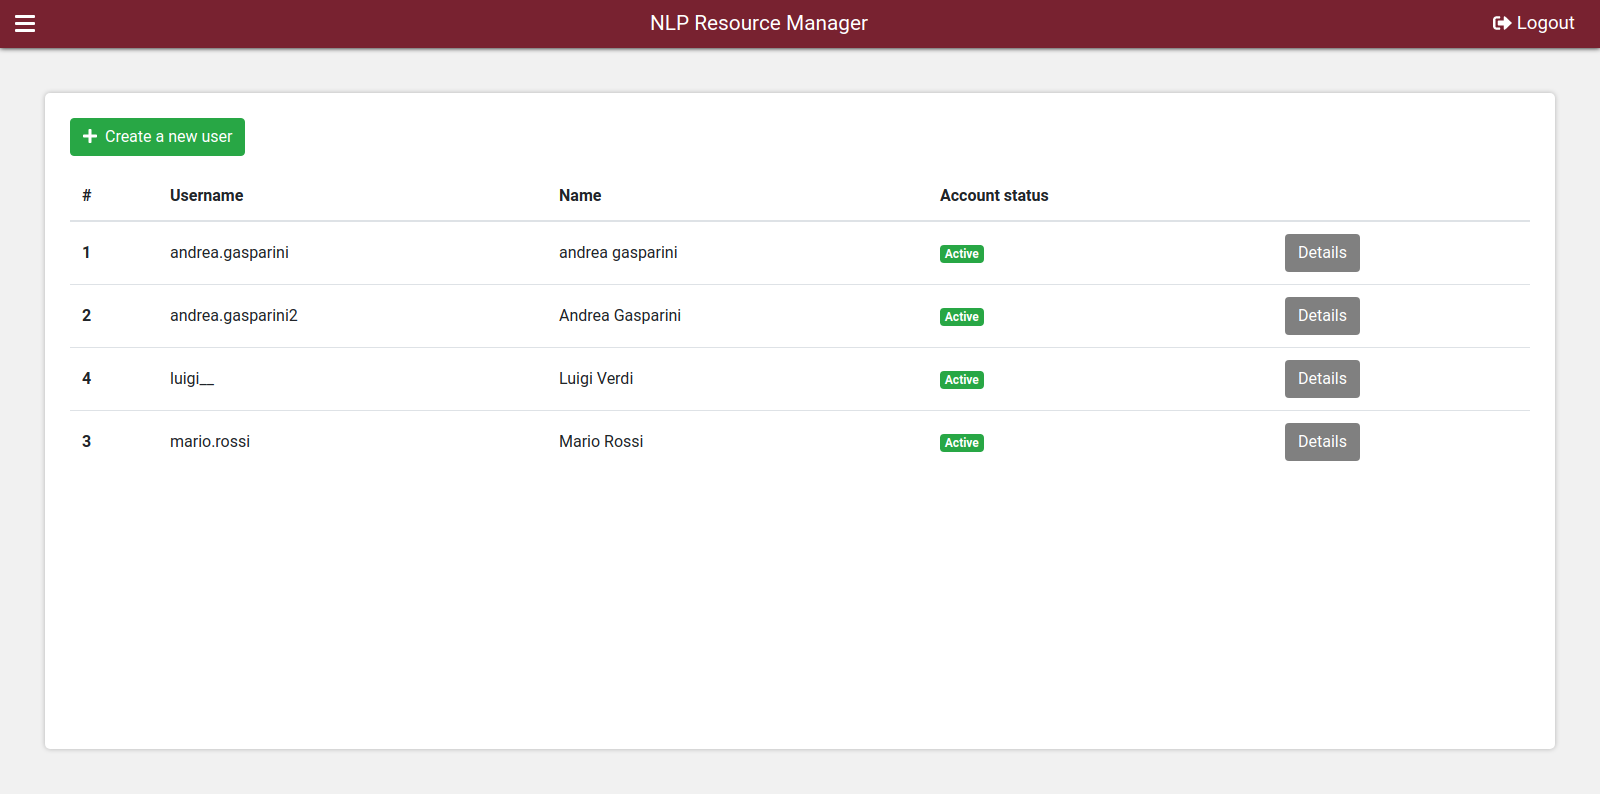
\includegraphics[width=\textwidth]{assets/ui/users-list.png}
	\caption{Resoconto degli utenti registrati}
	\label{fig:users-list}
\end{figure}

\begin{figure}[H]
	\centering
	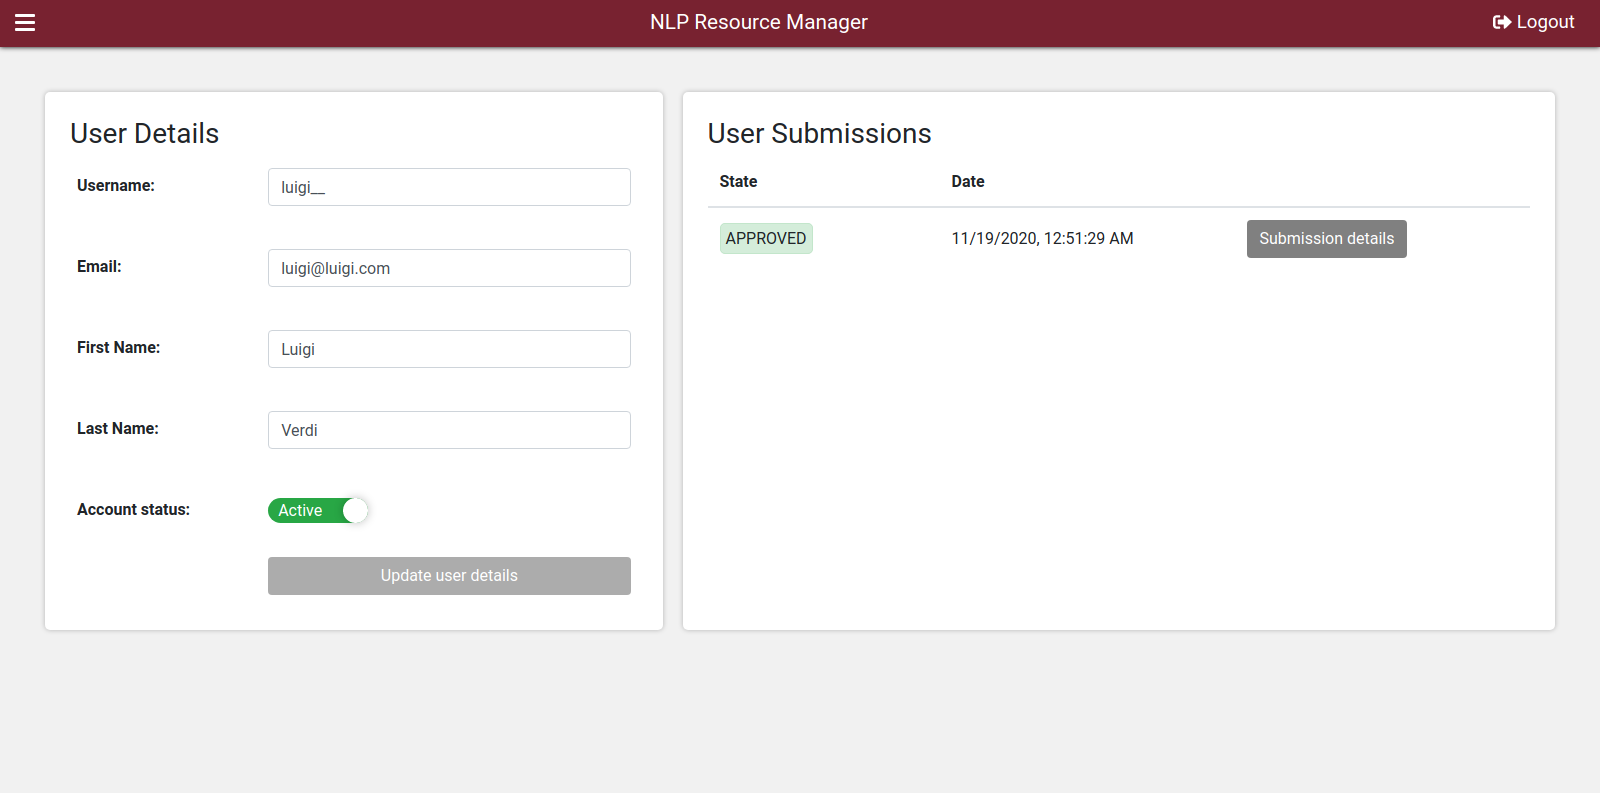
\includegraphics[width=\textwidth]{assets/ui/user-details.png}
	\caption{Dettaglio di un utente}
	\label{fig:user-details}
\end{figure}

\subsubsection{Gestione delle risorse}
In queste schermate è stata implementata la gestione dell'elemento cardine della
piattaforma, ovvero le risorse. Nel resoconto generale vengono mostrate le risorse
registrate nel database con nome e descrizione, oltre alla possibilità di crearne
di nuove. La selezione di una di esse permette di accedere al dettaglio, in cui
è possibile modificarne i dati, eliminarla definitivamente e aggiungervi una nuova
versione o modificare quelle disponibili.

\begin{figure}[H]
	\centering
	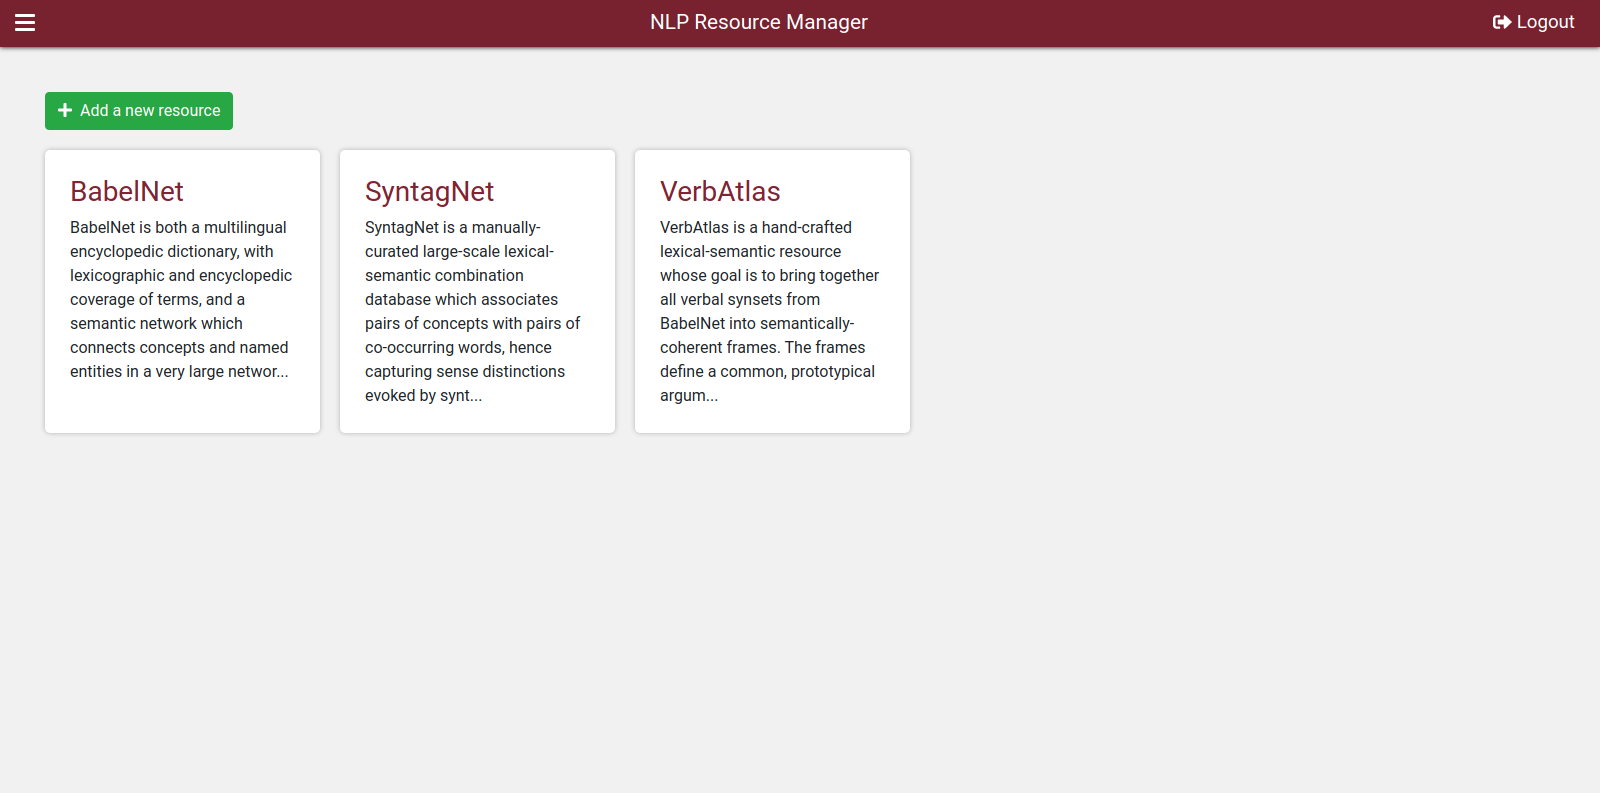
\includegraphics[width=\textwidth]{assets/ui/resources-list.png}
	\caption{Resoconto delle risorse disponibili}
	\label{fig:resources-list}
\end{figure}

\begin{figure}[H]
	\centering
	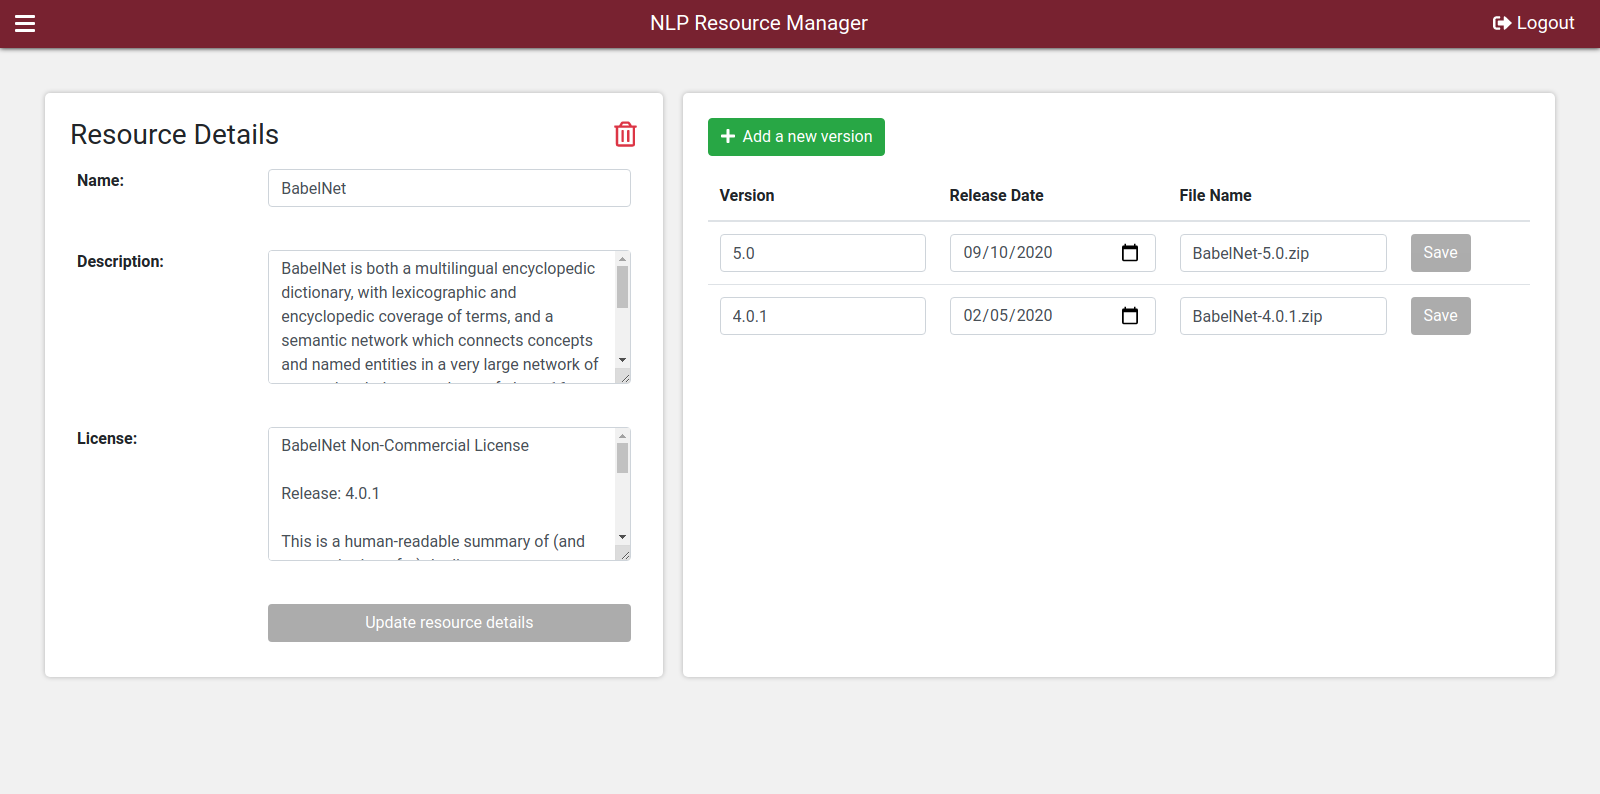
\includegraphics[width=\textwidth]{assets/ui/resource-details.png}
	\caption{Dettaglio di una risorsa}
	\label{fig:resource-details}
\end{figure}